\newpage
\section{Formulas}\label{app:formulas}
In this section the equations for calculation the area, water width and flow in a pipe will be shown.
%\begin{tikzpicture}

\draw  [ultra thick](-3.5,3) node (v9) {} ellipse (8.5 and 8.5);
\node (v1) at (-12,13.5) {};
\node (v2) at (5,13.5) {};
\draw  [ultra thick](v1) edge (v2);

\node (v3) at (-11.5,14) {};
\node (v4) at (-11.5,13) {};
\draw  [ultra thick](v3) edge (v1);
\draw  [ultra thick](v1) edge (v4);
\node (v5) at (4.5,14) {};
\node (v6) at (4.5,13) {};
\draw  [ultra thick](v5) edge (v2);
\draw  [ultra thick](v6) edge (v2);
\node (v8) at (-10,-2.5) {};
\node (v7) at (3,-2.5) {};
\draw  [ultra thick](v7) edge (v8);
\draw  [ultra thick](v8) edge (v9);
\draw  [ultra thick](v9) edge (v7);


\node (v11) at (6,-5.5) {};
\node (v10) at (6,-2.5) {};
\node (v14) at (5.5,-3) {};
\node (v15) at (6.5,-3) {};
\node (v12) at (5.5,-5) {};
\node (v13) at (6.5,-5) {};
\draw  [ultra thick](v10) edge (v11);
\draw  [ultra thick](v11) edge (v12);
\draw  [ultra thick](v11) edge (v13);
\draw  [ultra thick](v14) edge (v10);
\draw  [ultra thick](v10) edge (v15);


\draw [ultra thick](-4.6491,2.0358) arc (-140.0003:-40:1.5);
\node (v16) at (-9.5,-6) {};
\node (v19) at (3,-6.5) {};
\node (v21) at (2.5,-6) {};
\node (v20) at (2.5,-7) {};
\node (v17) at (-10,-6.5) {};
\node (v18) at (-9.5,-7) {};
\draw  [ultra thick](v16) edge (v17);
\draw  [ultra thick](v18) edge (v17);
\draw  [ultra thick](v19) edge (v17);
\draw  [ultra thick](v20) edge (v19);
\draw  [ultra thick](v21) edge (v19);
\draw  [ultra thick](v8) edge (v7);
\draw  [ultra thick](v7) edge (v8);
\draw  [ultra thick](v8) edge (v7);
\draw  [ultra thick](v7) edge (v9);
\draw  [ultra thick](v8) edge (v9);

%\draw  (-3.7,0.8) {theta}

\node  at (-3.5,1) {\Huge $\Theta$};
\node at (-4,14) {\Huge D};
\node at (6.5,-4) {\Huge h};
\node at (-3.5,-7) {\Huge B};
\end{tikzpicture}


In figure \ref{fig:calc_water_pipe_width} a illustration a cross view of a circular pipe is shown
\begin{figure}[H]
	\centering
	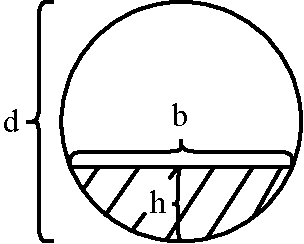
\includegraphics[width=0.20\textheight]{report/appendix/figures/calc_water_pipe_width.pdf}
	\caption{Cross section view of a circular pipe. Where d is the diameter, b is the width of the water in a given height, h is the height and the crossed section in the bottom illustrates the area of the water in the pipe.}
	\label{fig:calc_water_pipe_width}
\end{figure}

The area of the water in a circular pipe is calculated with the following \cite{ikke_stationear}: 
\begin{equation}%\label{eq:calc_area_open_channel}
	A = \frac {d^2}{4} \cdot acos \left(\frac{\frac{d}{2}-h}{\frac{d}{2}}\right)-\sqrt{h\cdot (d-h)}\cdot  \left(\frac{d}{2}-h\right)
\end{equation}

The water width in a pipe to a given height is calculated with the following equation \cite{ikke_stationear}:
\begin{equation}
	b = 2 \cdot \sqrt{-h+h\cdot d}
\end{equation}

The flow in a filled pipe can be calculated as \cite{ikke_stationear}:
\begin{equation}%\label{eq:qf_for_flow}
	Q_f =-72\cdot \left(\frac{d}{4}\right)^{0.635}\pi\cdot\left(\frac{d}{2}\right)^2\cdot I_e^{0,5}% -3.02 \cdot ln\left(\frac{0.74\cdot 10^{-6}}{d\sqrt{d\cdot I_e}}+\frac{k}{3.71\cdot d}\right)d^2\sqrt{d\cdot I_e}
\end{equation}
Where $I_e$ is a friction term. 

The flow in a pipe given a height can be calculated with the following equation \cite{ikke_stationear}:
\begin{equation}%\label{eq:calc_for_flowv2}
 	Q = \left(0.46-0.5 \cdot cos\left(\pi \frac{h}{d}\right)+0.04\cdot cos\left(2\pi\frac{h}{d}\right)\right)\cdot Q_f
\end{equation}

